% \begin{figure}[t]
% \centering
% \vspace*{-0.3cm}
% \begin{minipage}[b]{.4\linewidth}
% \centering
% 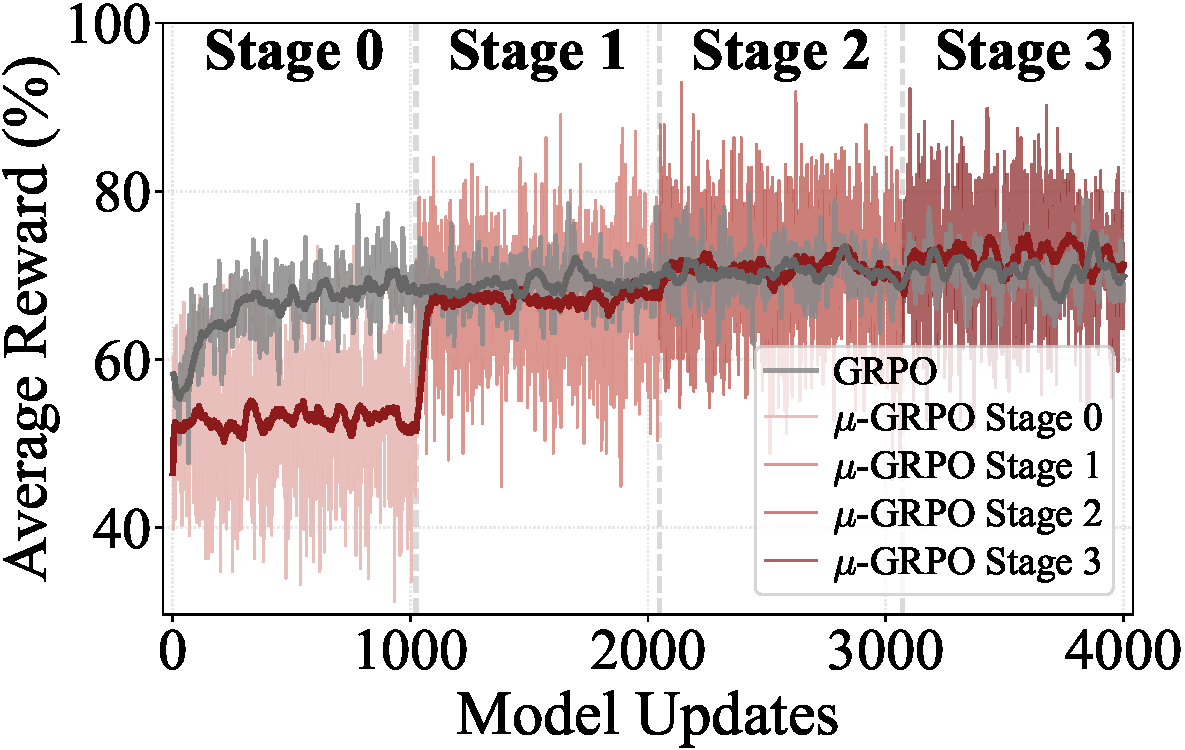
\includegraphics[width=\linewidth]{figures/reward.pdf}
% \end{minipage}
% \hfill
% \begin{minipage}[b]{.48\linewidth}
% \centering
% \caption{
% \textbf{Training-set reward dynamics} over 4096 model updates for GRPO
% ($\mu=4$) and \ourmethod{} ($\mu=1024$) on DeepSeek-7B, from the same run as
% Figure~\ref{fig:teaser}. Bold curves denote smoothed rewards. Despite high
% within-stage staleness, \ourmethod{} steadily improves reward, closely tracking
% the GRPO baseline, with larger variance but stable overall learning.
% }
% \label{fig:reward}
% \end{minipage}
% \vspace{-12pt}
% \end{figure}



\begin{figure}[t]
\centering
\vspace*{-0.3cm}
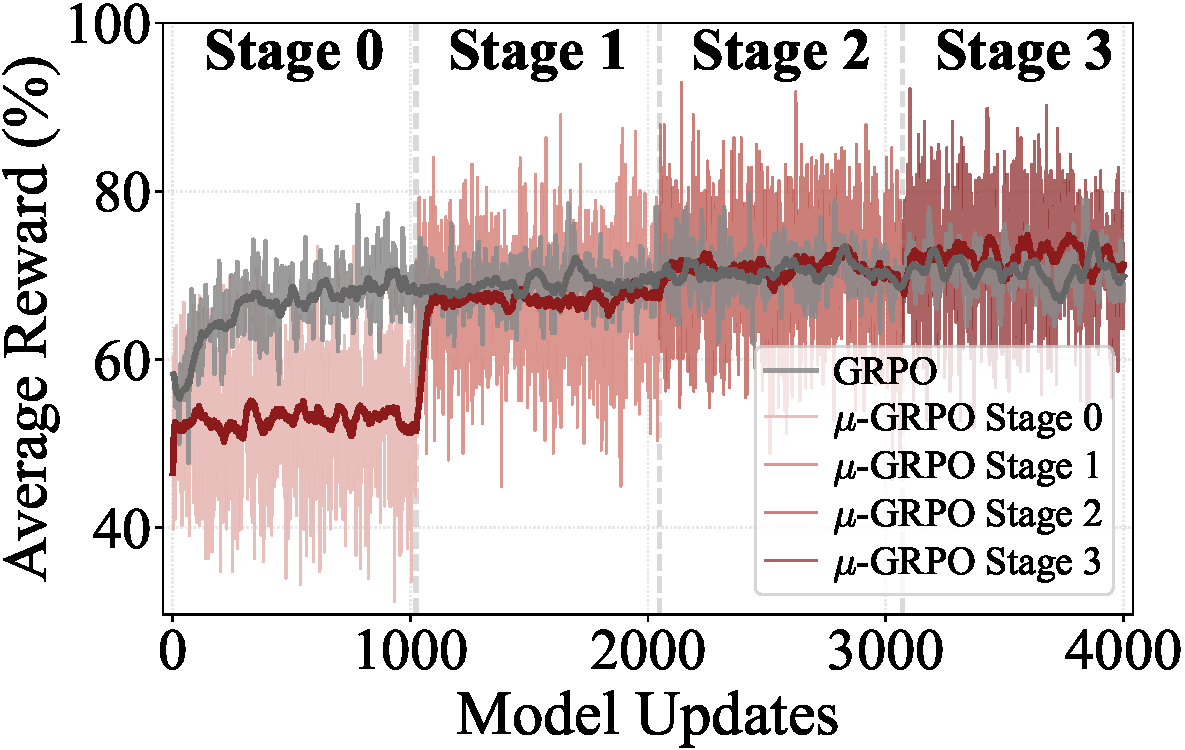
\includegraphics[width=0.6\linewidth]{figures/reward.pdf}
\caption{
\textbf{Training-set reward dynamics} over 4096 model updates for GRPO
($\mu=4$) and \ourmethod{} ($\mu=1024$) on DeepSeek-7B. Bold curves denote
smoothed rewards. \ourmethod{} maintains stable reward improvement across stages
despite larger variance from high rollout staleness.
}
\label{fig:reward}
\vspace{-12pt}
\end{figure}